\documentclass{article}
\usepackage{pgfplots}
\pgfplotsset{compat=1.18}

\begin{document}

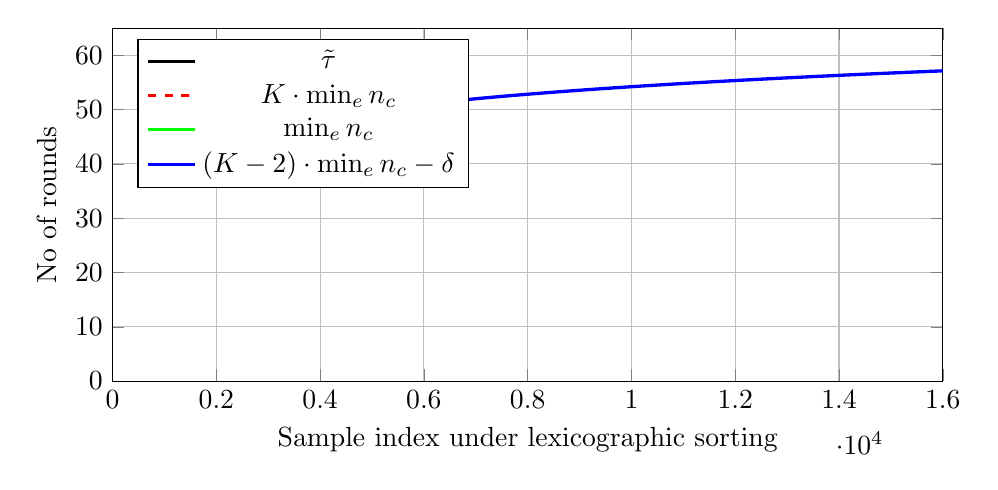
\begin{tikzpicture}
    \begin{axis}[
        xlabel={Sample index under lexicographic sorting},
        ylabel={No of rounds},
        xmin=0, xmax=1.6e4,
        ymin=0, ymax=65,
        xtick distance=0.2e4,
        ytick distance=10,
        legend pos=north west,
        grid=major,
        width=\textwidth,
        height=0.5\textwidth,
        smooth,
        mark size=1pt,
        ]
        % Black line
        \addplot [black, very thick, domain=0:1.6e4]
            {50 * log2(x) / log2(5)};
        \addlegendentry{$\tilde{\tau}$}

        % Red dashed line
        \addplot [red, dashed, very thick, domain=0:1.6e4]
            {100 * log2(x) / log2(5) + 5};
        \addlegendentry{$K \cdot \min_e n_c$}

        % Green solid line
        \addplot [green, very thick, domain=0:1.6e4]
            {20 * log2(x) / log2(5)};
        \addlegendentry{$\min_e n_c$}

        % Blue solid line
        \addplot [blue, very thick, domain=0:1.6e4]
            {(10 * log2(x) / log2(5)) - 3};
        \addlegendentry{$(K-2) \cdot \min_e n_c - \delta$}
    \end{axis}
\end{tikzpicture}

\caption{Measured $\hat{\tau}$ on all tuples from $\mathcal{S}(5, 60)$. The blue and green lines that were dashed in the previous figures have been made continuous to make clearer that the blue curve surpasses the green one.}

\end{document}